\documentclass[twoside]{article}

% Packages required by doxygen
\usepackage{fixltx2e}
\usepackage{calc}
\usepackage{doxygen}
\usepackage[export]{adjustbox} % also loads graphicx
\usepackage{graphicx}
\usepackage[utf8]{inputenc}
\usepackage{makeidx}
\usepackage{multicol}
\usepackage{multirow}
\PassOptionsToPackage{warn}{textcomp}
\usepackage{textcomp}
\usepackage[nointegrals]{wasysym}
\usepackage[table]{xcolor}

% NLS support packages
\usepackage{polski}
\usepackage[T1]{fontenc}

% Font selection
\usepackage[T1]{fontenc}
\usepackage[scaled=.90]{helvet}
\usepackage{courier}
\usepackage{amssymb}
\usepackage{sectsty}
\renewcommand{\familydefault}{\sfdefault}
\allsectionsfont{%
  \fontseries{bc}\selectfont%
  \color{darkgray}%
}
\renewcommand{\DoxyLabelFont}{%
  \fontseries{bc}\selectfont%
  \color{darkgray}%
}
\newcommand{\+}{\discretionary{\mbox{\scriptsize$\hookleftarrow$}}{}{}}

% Page & text layout
\usepackage{geometry}
\geometry{%
  a4paper,%
  top=2.5cm,%
  bottom=2.5cm,%
  left=2.5cm,%
  right=2.5cm%
}
\tolerance=750
\hfuzz=15pt
\hbadness=750
\setlength{\emergencystretch}{15pt}
\setlength{\parindent}{0cm}
\setlength{\parskip}{0.2cm}
\makeatletter
\renewcommand{\paragraph}{%
  \@startsection{paragraph}{4}{0ex}{-1.0ex}{1.0ex}{%
    \normalfont\normalsize\bfseries\SS@parafont%
  }%
}
\renewcommand{\subparagraph}{%
  \@startsection{subparagraph}{5}{0ex}{-1.0ex}{1.0ex}{%
    \normalfont\normalsize\bfseries\SS@subparafont%
  }%
}
\makeatother

% Headers & footers
\usepackage{fancyhdr}
\pagestyle{fancyplain}
\fancyhead[LE]{\fancyplain{}{\bfseries\thepage}}
\fancyhead[CE]{\fancyplain{}{}}
\fancyhead[RE]{\fancyplain{}{\bfseries\leftmark}}
\fancyhead[LO]{\fancyplain{}{\bfseries\rightmark}}
\fancyhead[CO]{\fancyplain{}{}}
\fancyhead[RO]{\fancyplain{}{\bfseries\thepage}}
\fancyfoot[LE]{\fancyplain{}{}}
\fancyfoot[CE]{\fancyplain{}{}}
\fancyfoot[RE]{\fancyplain{}{\bfseries\scriptsize Wygenerowano Śr, 18 mar 2015 11\+:45\+:35 dla Program framework benchmarkujacy dla struktur danych Stos, Lista i Kolejka -\/ Laboratorium 2 programem Doxygen }}
\fancyfoot[LO]{\fancyplain{}{\bfseries\scriptsize Wygenerowano Śr, 18 mar 2015 11\+:45\+:35 dla Program framework benchmarkujacy dla struktur danych Stos, Lista i Kolejka -\/ Laboratorium 2 programem Doxygen }}
\fancyfoot[CO]{\fancyplain{}{}}
\fancyfoot[RO]{\fancyplain{}{}}
\renewcommand{\footrulewidth}{0.4pt}
\renewcommand{\sectionmark}[1]{%
  \markright{\thesection\ #1}%
}

% Indices & bibliography
\usepackage{natbib}
\usepackage[titles]{tocloft}
\setcounter{tocdepth}{3}
\setcounter{secnumdepth}{5}
\makeindex

% Hyperlinks (required, but should be loaded last)
\usepackage{ifpdf}
\ifpdf
  \usepackage[pdftex,pagebackref=true]{hyperref}
\else
  \usepackage[ps2pdf,pagebackref=true]{hyperref}
\fi
\hypersetup{%
  colorlinks=true,%
  linkcolor=blue,%
  citecolor=blue,%
  unicode%
}

% Custom commands
\newcommand{\clearemptydoublepage}{%
  \newpage{\pagestyle{empty}\cleardoublepage}%
}


%===== C O N T E N T S =====

\begin{document}

% Titlepage & ToC
\hypersetup{pageanchor=false,
             bookmarks=true,
             bookmarksnumbered=true,
             pdfencoding=unicode
            }
\pagenumbering{roman}
\begin{titlepage}
\vspace*{7cm}
\begin{center}%
{\Large Program framework benchmarkujacy dla struktur danych Stos, Lista i Kolejka -\/ Laboratorium 2 }\\
\vspace*{1cm}
{\large Wygenerowano przez Doxygen 1.8.9.1}\\
\vspace*{0.5cm}
{\small Śr, 18 mar 2015 11:45:35}\\
\end{center}
\end{titlepage}
\tableofcontents
\pagenumbering{arabic}
\hypersetup{pageanchor=true}

%--- Begin generated contents ---
\section{Program framework benchmarkujacy dla struktur danych Stos, Lista i Kolejka}
\label{index}\hypertarget{index}{}\begin{DoxyAuthor}{Autor}
Wojcich Makuch 
\end{DoxyAuthor}
\begin{DoxyDate}{Data}
10.\+03.\+2015 
\end{DoxyDate}
\begin{DoxyVersion}{Wersja}
1.\+0
\end{DoxyVersion}
Zadaniem programu jest wygenerowanie tablic liczb pseldoloswych oraz pomiar zlozonosci obliczeniowej polegajacej na wymnozeniu kazdego z tych elementow przez 2. Program zapisuje dane w pliku o nazwie Pomiar\+Czasu1.\+txt.\hypertarget{index_wartosci}{}\subsection{wartosci}\label{index_wartosci}
Program wykonuje obliczenia dla tablic o rozmiarach\+: 10 50 1e02 5e02 1e03 5e03 1e04 5e04 1e06 2.\+5e06 5e06 7.\+5e06 1e07 5e07 1e08 2.\+5e08 
\section{Indeks klas}
\subsection{Lista klas}
Tutaj znajdują się klasy, struktury, unie i interfejsy wraz z ich krótkimi opisami\+:\begin{DoxyCompactList}
\item\contentsline{section}{\hyperlink{class_kolejka}{Kolejka$<$ typ $>$} \\*Definicja klasy \hyperlink{class_kolejka}{Kolejka} Zbudowana na tablicy posiada indeksy pokazujace na poczatek i na koniec kolejki. Zbudowana na szablonie }{\pageref{class_kolejka}}{}
\item\contentsline{section}{\hyperlink{class_lista}{Lista$<$ typ $>$} \\*Definicja klasy \hyperlink{class_lista}{Lista} Przechowuje obiekt oraz wskaznik na nastepny i pole rozmiar. Zbudowana na szablonie }{\pageref{class_lista}}{}
\item\contentsline{section}{\hyperlink{class_stos}{Stos$<$ typ $>$} \\*Definicja klasy \hyperlink{class_stos}{Stos} zedfiniowany za pomoca tablicy. Klasa zbudowana na szablonie }{\pageref{class_stos}}{}
\end{DoxyCompactList}

\section{Dokumentacja klas}
\hypertarget{class_kolejka}{}\subsection{Dokumentacja szablonu klasy Kolejka$<$ typ $>$}
\label{class_kolejka}\index{Kolejka$<$ typ $>$@{Kolejka$<$ typ $>$}}


definicja klasy \hyperlink{class_kolejka}{Kolejka} Zbudowana na tablicy posiada indeksy pokazujace na poczatek i na koniec kolejki. Zbudowana na szablonie.  




{\ttfamily \#include $<$Kolejka.\+hh$>$}

\subsubsection*{Metody publiczne}
\begin{DoxyCompactItemize}
\item 
\hyperlink{class_kolejka_a9e3a347692b91c7c805dbc4c600d3611}{Kolejka} (int ilosc)
\begin{DoxyCompactList}\small\item\em definicja konstruktora z jednym parametrem \end{DoxyCompactList}\item 
\hyperlink{class_kolejka_ae64d506b36a27fdf2c66e53aaa7ae79d}{Kolejka} ()
\begin{DoxyCompactList}\small\item\em definicja konstruktora bezparametrycznego Zeruje rozmiar, ustawia wskaznik tablicy na N\+U\+L\+L, zeruje indeksy. \end{DoxyCompactList}\item 
\hyperlink{class_kolejka_a19d3261c05d90a58feed8340ea995258}{$\sim$\+Kolejka} ()
\begin{DoxyCompactList}\small\item\em definicja destruktora Zwalnia zaalokowana pamiec tablicy. Zeruje indeksy i rozmiar. \end{DoxyCompactList}\item 
int \hyperlink{class_kolejka_a487b41717feb173ed0cac156d143a7f9}{size} () const 
\begin{DoxyCompactList}\small\item\em definicja metody size \end{DoxyCompactList}\item 
void \hyperlink{class_kolejka_a8cf2fbf3b641c1914d63580ce59ec3ef}{enqueue} (typ element)
\begin{DoxyCompactList}\small\item\em definicja metody enqueue \end{DoxyCompactList}\item 
typ \hyperlink{class_kolejka_a7473ad1afce6acba353bfdd78f7c72e0}{dequeue} ()
\begin{DoxyCompactList}\small\item\em definicja metody dequeue \end{DoxyCompactList}\end{DoxyCompactItemize}
\subsubsection*{Atrybuty prywatne}
\begin{DoxyCompactItemize}
\item 
int \hyperlink{class_kolejka_aa533196e5ca1ca0033142a1588000edd}{f}
\item 
int \hyperlink{class_kolejka_aa26f38fd232737021fb82f5d8e86c724}{r}
\item 
typ $\ast$ \hyperlink{class_kolejka_a333beaaaf8ccecbfd4b84a7840d3bd33}{tab}
\item 
int \hyperlink{class_kolejka_a031fd520e5f22daac808dbeeb705832a}{rozmiar}
\end{DoxyCompactItemize}


\subsubsection{Opis szczegółowy}
\subsubsection*{template$<$typename typ$>$class Kolejka$<$ typ $>$}

definicja klasy \hyperlink{class_kolejka}{Kolejka} Zbudowana na tablicy posiada indeksy pokazujace na poczatek i na koniec kolejki. Zbudowana na szablonie. 

Definicja w linii 16 pliku Kolejka.\+hh.



\subsubsection{Dokumentacja konstruktora i destruktora}
\hypertarget{class_kolejka_a9e3a347692b91c7c805dbc4c600d3611}{}\index{Kolejka@{Kolejka}!Kolejka@{Kolejka}}
\index{Kolejka@{Kolejka}!Kolejka@{Kolejka}}
\paragraph[{Kolejka}]{\setlength{\rightskip}{0pt plus 5cm}template$<$typename typ $>$ {\bf Kolejka}$<$ typ $>$\+::{\bf Kolejka} (
\begin{DoxyParamCaption}
\item[{int}]{ilosc}
\end{DoxyParamCaption}
)}\label{class_kolejka_a9e3a347692b91c7c805dbc4c600d3611}


definicja konstruktora z jednym parametrem 

max rozmiar tablicy


\begin{DoxyParams}{Parametry}
{\em \mbox{[}ilosc\mbox{]}} & rozmiar alokowanej tablicy Alokuje tablice o zadanym rozmiarze. Ustawia indeksy na 0. \\
\hline
\end{DoxyParams}


Definicja w linii 37 pliku Kolejka.\+hh.

\hypertarget{class_kolejka_ae64d506b36a27fdf2c66e53aaa7ae79d}{}\index{Kolejka@{Kolejka}!Kolejka@{Kolejka}}
\index{Kolejka@{Kolejka}!Kolejka@{Kolejka}}
\paragraph[{Kolejka}]{\setlength{\rightskip}{0pt plus 5cm}template$<$typename typ $>$ {\bf Kolejka}$<$ typ $>$\+::{\bf Kolejka} (
\begin{DoxyParamCaption}
{}
\end{DoxyParamCaption}
)}\label{class_kolejka_ae64d506b36a27fdf2c66e53aaa7ae79d}


definicja konstruktora bezparametrycznego Zeruje rozmiar, ustawia wskaznik tablicy na N\+U\+L\+L, zeruje indeksy. 



Definicja w linii 50 pliku Kolejka.\+hh.

\hypertarget{class_kolejka_a19d3261c05d90a58feed8340ea995258}{}\index{Kolejka@{Kolejka}!````~Kolejka@{$\sim$\+Kolejka}}
\index{````~Kolejka@{$\sim$\+Kolejka}!Kolejka@{Kolejka}}
\paragraph[{$\sim$\+Kolejka}]{\setlength{\rightskip}{0pt plus 5cm}template$<$typename typ $>$ {\bf Kolejka}$<$ typ $>$\+::$\sim${\bf Kolejka} (
\begin{DoxyParamCaption}
{}
\end{DoxyParamCaption}
)}\label{class_kolejka_a19d3261c05d90a58feed8340ea995258}


definicja destruktora Zwalnia zaalokowana pamiec tablicy. Zeruje indeksy i rozmiar. 



Definicja w linii 63 pliku Kolejka.\+hh.



\subsubsection{Dokumentacja funkcji składowych}
\hypertarget{class_kolejka_a7473ad1afce6acba353bfdd78f7c72e0}{}\index{Kolejka@{Kolejka}!dequeue@{dequeue}}
\index{dequeue@{dequeue}!Kolejka@{Kolejka}}
\paragraph[{dequeue}]{\setlength{\rightskip}{0pt plus 5cm}template$<$typename typ $>$ typ {\bf Kolejka}$<$ typ $>$\+::dequeue (
\begin{DoxyParamCaption}
{}
\end{DoxyParamCaption}
)}\label{class_kolejka_a7473ad1afce6acba353bfdd78f7c72e0}


definicja metody dequeue 

\begin{DoxyReturn}{Zwraca}
element z poczatku kolejki 

0 i wyswietla komunikat gdy kolejka jest pusta. zmienia polozenie indeksu poczatku. 
\end{DoxyReturn}


Definicja w linii 125 pliku Kolejka.\+hh.

\hypertarget{class_kolejka_a8cf2fbf3b641c1914d63580ce59ec3ef}{}\index{Kolejka@{Kolejka}!enqueue@{enqueue}}
\index{enqueue@{enqueue}!Kolejka@{Kolejka}}
\paragraph[{enqueue}]{\setlength{\rightskip}{0pt plus 5cm}template$<$typename typ $>$ void {\bf Kolejka}$<$ typ $>$\+::enqueue (
\begin{DoxyParamCaption}
\item[{typ}]{element}
\end{DoxyParamCaption}
)}\label{class_kolejka_a8cf2fbf3b641c1914d63580ce59ec3ef}


definicja metody enqueue 


\begin{DoxyParams}{Parametry}
{\em \mbox{[}element\mbox{]}} & dodawany element Dodaje element na koniec kolejki. Gdy kolejka jest pelna, powieksza tablice o 5 i przekopiowywuje elementy. zmienia polozenie indeksu konca. \\
\hline
\end{DoxyParams}


Definicja w linii 91 pliku Kolejka.\+hh.

\hypertarget{class_kolejka_a487b41717feb173ed0cac156d143a7f9}{}\index{Kolejka@{Kolejka}!size@{size}}
\index{size@{size}!Kolejka@{Kolejka}}
\paragraph[{size}]{\setlength{\rightskip}{0pt plus 5cm}template$<$typename typ $>$ int {\bf Kolejka}$<$ typ $>$\+::size (
\begin{DoxyParamCaption}
{}
\end{DoxyParamCaption}
) const}\label{class_kolejka_a487b41717feb173ed0cac156d143a7f9}


definicja metody size 

\begin{DoxyReturn}{Zwraca}
rozmiar ilosci danych przechowywanych w tablicy. 

0, gdy kolejka jest pusta. 
\end{DoxyReturn}


Definicja w linii 75 pliku Kolejka.\+hh.



\subsubsection{Dokumentacja atrybutów składowych}
\hypertarget{class_kolejka_aa533196e5ca1ca0033142a1588000edd}{}\index{Kolejka@{Kolejka}!f@{f}}
\index{f@{f}!Kolejka@{Kolejka}}
\paragraph[{f}]{\setlength{\rightskip}{0pt plus 5cm}template$<$typename typ$>$ int {\bf Kolejka}$<$ typ $>$\+::f\hspace{0.3cm}{\ttfamily [private]}}\label{class_kolejka_aa533196e5ca1ca0033142a1588000edd}


Definicja w linii 17 pliku Kolejka.\+hh.

\hypertarget{class_kolejka_aa26f38fd232737021fb82f5d8e86c724}{}\index{Kolejka@{Kolejka}!r@{r}}
\index{r@{r}!Kolejka@{Kolejka}}
\paragraph[{r}]{\setlength{\rightskip}{0pt plus 5cm}template$<$typename typ$>$ int {\bf Kolejka}$<$ typ $>$\+::r\hspace{0.3cm}{\ttfamily [private]}}\label{class_kolejka_aa26f38fd232737021fb82f5d8e86c724}
poczatek 

Definicja w linii 18 pliku Kolejka.\+hh.

\hypertarget{class_kolejka_a031fd520e5f22daac808dbeeb705832a}{}\index{Kolejka@{Kolejka}!rozmiar@{rozmiar}}
\index{rozmiar@{rozmiar}!Kolejka@{Kolejka}}
\paragraph[{rozmiar}]{\setlength{\rightskip}{0pt plus 5cm}template$<$typename typ$>$ int {\bf Kolejka}$<$ typ $>$\+::rozmiar\hspace{0.3cm}{\ttfamily [private]}}\label{class_kolejka_a031fd520e5f22daac808dbeeb705832a}
przechowywane elementy 

Definicja w linii 20 pliku Kolejka.\+hh.

\hypertarget{class_kolejka_a333beaaaf8ccecbfd4b84a7840d3bd33}{}\index{Kolejka@{Kolejka}!tab@{tab}}
\index{tab@{tab}!Kolejka@{Kolejka}}
\paragraph[{tab}]{\setlength{\rightskip}{0pt plus 5cm}template$<$typename typ$>$ typ$\ast$ {\bf Kolejka}$<$ typ $>$\+::tab\hspace{0.3cm}{\ttfamily [private]}}\label{class_kolejka_a333beaaaf8ccecbfd4b84a7840d3bd33}
koniec 

Definicja w linii 19 pliku Kolejka.\+hh.


\hypertarget{class_lista}{}\subsection{Dokumentacja szablonu klasy Lista$<$ typ $>$}
\label{class_lista}\index{Lista$<$ typ $>$@{Lista$<$ typ $>$}}


definicja klasy \hyperlink{class_lista}{Lista} Przechowuje obiekt oraz wskaznik na nastepny i pole rozmiar. Zbudowana na szablonie.  




{\ttfamily \#include $<$Lista.\+hh$>$}

\subsubsection*{Metody publiczne}
\begin{DoxyCompactItemize}
\item 
\hyperlink{class_lista_a23a5b3313a893057276942e74f330b89}{Lista} ()
\begin{DoxyCompactList}\small\item\em definicja konstruktora bezparametrycznego Zeruje rozmiar, ustawia wskaznik na N\+U\+L\+L. \end{DoxyCompactList}\item 
\hyperlink{class_lista_accc5a3585c7f97372f35f81ef574646e}{$\sim$\+Lista} ()
\begin{DoxyCompactList}\small\item\em definicja destruktora Zeruje rozmiar, Kasuje wszystkie obiektry/elementy. \end{DoxyCompactList}\item 
void \hyperlink{class_lista_afe3d2ff8a9161d30301bfc210287ab51}{push} (typ element)
\begin{DoxyCompactList}\small\item\em definicja metody push \end{DoxyCompactList}\item 
typ \hyperlink{class_lista_a536acf0c981ac359d145da0cc452aadf}{pop} ()
\begin{DoxyCompactList}\small\item\em definicja metody pop \end{DoxyCompactList}\item 
int \hyperlink{class_lista_a8025f28bcc402832d854af6b874451f1}{size} () const 
\begin{DoxyCompactList}\small\item\em deinicja metody size \end{DoxyCompactList}\end{DoxyCompactItemize}
\subsubsection*{Atrybuty prywatne}
\begin{DoxyCompactItemize}
\item 
\hyperlink{class_lista}{Lista}$<$ typ $>$ $\ast$ \hyperlink{class_lista_a42fc5a822a0f442758c88cbf1e19d15f}{nastepny}
\item 
typ \hyperlink{class_lista_a017ecd407cac7e93841f69280f4caa1a}{dane}
\item 
int \hyperlink{class_lista_a5b9d349b6ba27b55058ca77cb0909b6e}{rozmiar}
\end{DoxyCompactItemize}


\subsubsection{Opis szczegółowy}
\subsubsection*{template$<$typename typ$>$class Lista$<$ typ $>$}



Definicja w linii 15 pliku Lista.\+hh.



\subsubsection{Dokumentacja konstruktora i destruktora}
\hypertarget{class_lista_a23a5b3313a893057276942e74f330b89}{}\index{Lista@{Lista}!Lista@{Lista}}
\index{Lista@{Lista}!Lista@{Lista}}
\paragraph[{Lista}]{\setlength{\rightskip}{0pt plus 5cm}template$<$typename typ $>$ {\bf Lista}$<$ typ $>$\+::{\bf Lista} (
\begin{DoxyParamCaption}
{}
\end{DoxyParamCaption}
)}\label{class_lista_a23a5b3313a893057276942e74f330b89}
ilosc elementow/obiektow 

Definicja w linii 33 pliku Lista.\+hh.

\hypertarget{class_lista_accc5a3585c7f97372f35f81ef574646e}{}\index{Lista@{Lista}!````~Lista@{$\sim$\+Lista}}
\index{````~Lista@{$\sim$\+Lista}!Lista@{Lista}}
\paragraph[{$\sim$\+Lista}]{\setlength{\rightskip}{0pt plus 5cm}template$<$typename typ $>$ {\bf Lista}$<$ typ $>$\+::$\sim${\bf Lista} (
\begin{DoxyParamCaption}
{}
\end{DoxyParamCaption}
)}\label{class_lista_accc5a3585c7f97372f35f81ef574646e}


Definicja w linii 94 pliku Lista.\+hh.



\subsubsection{Dokumentacja funkcji składowych}
\hypertarget{class_lista_a536acf0c981ac359d145da0cc452aadf}{}\index{Lista@{Lista}!pop@{pop}}
\index{pop@{pop}!Lista@{Lista}}
\paragraph[{pop}]{\setlength{\rightskip}{0pt plus 5cm}template$<$typename typ $>$ typ {\bf Lista}$<$ typ $>$\+::pop (
\begin{DoxyParamCaption}
{}
\end{DoxyParamCaption}
)}\label{class_lista_a536acf0c981ac359d145da0cc452aadf}
\begin{DoxyReturn}{Zwraca}
usuwany element Ustawia wskaznik na poprzedni element zwraca i kasuje ostatni element. 

0 i wyswietla komunikat gdy lista jest pusta. 
\end{DoxyReturn}


Definicja w linii 62 pliku Lista.\+hh.

\hypertarget{class_lista_afe3d2ff8a9161d30301bfc210287ab51}{}\index{Lista@{Lista}!push@{push}}
\index{push@{push}!Lista@{Lista}}
\paragraph[{push}]{\setlength{\rightskip}{0pt plus 5cm}template$<$typename typ $>$ void {\bf Lista}$<$ typ $>$\+::push (
\begin{DoxyParamCaption}
\item[{typ}]{element}
\end{DoxyParamCaption}
)}\label{class_lista_afe3d2ff8a9161d30301bfc210287ab51}

\begin{DoxyParams}{Parametry}
{\em \mbox{[}element\mbox{]}} & dodawany element na koniec listy Zwieksza rozmiar, alokuje pamiec, przypisuje element do pola klasy. \\
\hline
\end{DoxyParams}


Definicja w linii 45 pliku Lista.\+hh.

\hypertarget{class_lista_a8025f28bcc402832d854af6b874451f1}{}\index{Lista@{Lista}!size@{size}}
\index{size@{size}!Lista@{Lista}}
\paragraph[{size}]{\setlength{\rightskip}{0pt plus 5cm}template$<$typename typ $>$ int {\bf Lista}$<$ typ $>$\+::size (
\begin{DoxyParamCaption}
{}
\end{DoxyParamCaption}
) const}\label{class_lista_a8025f28bcc402832d854af6b874451f1}
\begin{DoxyReturn}{Zwraca}
ilosc elementow przechowywanych na liscie. 
\end{DoxyReturn}


Definicja w linii 83 pliku Lista.\+hh.



\subsubsection{Dokumentacja atrybutów składowych}
\hypertarget{class_lista_a017ecd407cac7e93841f69280f4caa1a}{}\index{Lista@{Lista}!dane@{dane}}
\index{dane@{dane}!Lista@{Lista}}
\paragraph[{dane}]{\setlength{\rightskip}{0pt plus 5cm}template$<$typename typ$>$ typ {\bf Lista}$<$ typ $>$\+::dane\hspace{0.3cm}{\ttfamily [private]}}\label{class_lista_a017ecd407cac7e93841f69280f4caa1a}
wskaznik na nastepny obiekt/element 

Definicja w linii 17 pliku Lista.\+hh.

\hypertarget{class_lista_a42fc5a822a0f442758c88cbf1e19d15f}{}\index{Lista@{Lista}!nastepny@{nastepny}}
\index{nastepny@{nastepny}!Lista@{Lista}}
\paragraph[{nastepny}]{\setlength{\rightskip}{0pt plus 5cm}template$<$typename typ$>$ {\bf Lista}$<$typ$>$$\ast$ {\bf Lista}$<$ typ $>$\+::nastepny\hspace{0.3cm}{\ttfamily [private]}}\label{class_lista_a42fc5a822a0f442758c88cbf1e19d15f}


Definicja w linii 16 pliku Lista.\+hh.

\hypertarget{class_lista_a5b9d349b6ba27b55058ca77cb0909b6e}{}\index{Lista@{Lista}!rozmiar@{rozmiar}}
\index{rozmiar@{rozmiar}!Lista@{Lista}}
\paragraph[{rozmiar}]{\setlength{\rightskip}{0pt plus 5cm}template$<$typename typ$>$ int {\bf Lista}$<$ typ $>$\+::rozmiar\hspace{0.3cm}{\ttfamily [private]}}\label{class_lista_a5b9d349b6ba27b55058ca77cb0909b6e}
przechowywana informacja/obiekt/element 

Definicja w linii 18 pliku Lista.\+hh.



Dokumentacja dla tej klasy została wygenerowana z pliku\+:\begin{DoxyCompactItemize}
\item 
\hyperlink{_lista_8hh}{Lista.\+hh}\end{DoxyCompactItemize}

\hypertarget{class_stos}{}\subsection{Dokumentacja szablonu klasy Stos$<$ typ $>$}
\label{class_stos}\index{Stos$<$ typ $>$@{Stos$<$ typ $>$}}


definicja klasy \hyperlink{class_stos}{Stos} zedfiniowany za pomoca tablicy. Klasa zbudowana na szablonie.  




{\ttfamily \#include $<$Stos.\+hh$>$}

\subsubsection*{Metody publiczne}
\begin{DoxyCompactItemize}
\item 
\hyperlink{class_stos_af6c53f2458ebd95fd992a14fef6712d0}{Stos} (typ p)
\begin{DoxyCompactList}\small\item\em definicja konstruktora z jednym parametrem \end{DoxyCompactList}\item 
\hyperlink{class_stos_afc525fb8a9f8f80fda9bf0f846c078c4}{Stos} ()
\begin{DoxyCompactList}\small\item\em definicja konstruktora bezparametrycznego zeruje rozmiar, przypisuje N\+U\+L\+L do wskaznikow. \end{DoxyCompactList}\item 
\hyperlink{class_stos_a1e9ba3ec6f2759c1fd9a69b56b0d0c5f}{$\sim$\+Stos} ()
\begin{DoxyCompactList}\small\item\em definicja destruktora Zwalnia pamiec, zeruje rozmiar. \end{DoxyCompactList}\item 
void \hyperlink{class_stos_a51e06002fe60a5946cb2dd82cd0c0e06}{push} (typ element)
\begin{DoxyCompactList}\small\item\em definicja metody push \end{DoxyCompactList}\item 
typ \hyperlink{class_stos_a779da9dd1daf1118cd4b213401a4e1ed}{pop} ()
\begin{DoxyCompactList}\small\item\em definicja metody pop zmmniejsza rozmiar o 1, \end{DoxyCompactList}\item 
int \hyperlink{class_stos_aedf6a4f76e7f0bce073a21be4db7163c}{size} () const 
\begin{DoxyCompactList}\small\item\em definicja metody size \end{DoxyCompactList}\end{DoxyCompactItemize}
\subsubsection*{Atrybuty prywatne}
\begin{DoxyCompactItemize}
\item 
int \hyperlink{class_stos_a66c92dc47edd280d9ea15fbcafcd9a80}{rozmiar}
\item 
typ $\ast$ \hyperlink{class_stos_acb9c6baeb0616796d20cfd05f6457fe3}{tab}
\end{DoxyCompactItemize}


\subsubsection{Opis szczegółowy}
\subsubsection*{template$<$typename typ$>$class Stos$<$ typ $>$}

definicja klasy \hyperlink{class_stos}{Stos} zedfiniowany za pomoca tablicy. Klasa zbudowana na szablonie. 

Definicja w linii 17 pliku Stos.\+hh.



\subsubsection{Dokumentacja konstruktora i destruktora}
\hypertarget{class_stos_af6c53f2458ebd95fd992a14fef6712d0}{}\index{Stos@{Stos}!Stos@{Stos}}
\index{Stos@{Stos}!Stos@{Stos}}
\paragraph[{Stos}]{\setlength{\rightskip}{0pt plus 5cm}template$<$typename typ $>$ {\bf Stos}$<$ typ $>$\+::{\bf Stos} (
\begin{DoxyParamCaption}
\item[{typ}]{p}
\end{DoxyParamCaption}
)}\label{class_stos_af6c53f2458ebd95fd992a14fef6712d0}


definicja konstruktora z jednym parametrem 

alokowana pamiec


\begin{DoxyParams}{Parametry}
{\em \mbox{[}p\mbox{]}} & rozmiar ilosci alokowanej pamieci alokuje pamiec o zadanym rozmiarze \\
\hline
\end{DoxyParams}


Definicja w linii 36 pliku Stos.\+hh.

\hypertarget{class_stos_afc525fb8a9f8f80fda9bf0f846c078c4}{}\index{Stos@{Stos}!Stos@{Stos}}
\index{Stos@{Stos}!Stos@{Stos}}
\paragraph[{Stos}]{\setlength{\rightskip}{0pt plus 5cm}template$<$typename typ $>$ {\bf Stos}$<$ typ $>$\+::{\bf Stos} (
\begin{DoxyParamCaption}
{}
\end{DoxyParamCaption}
)}\label{class_stos_afc525fb8a9f8f80fda9bf0f846c078c4}


definicja konstruktora bezparametrycznego zeruje rozmiar, przypisuje N\+U\+L\+L do wskaznikow. 



Definicja w linii 47 pliku Stos.\+hh.

\hypertarget{class_stos_a1e9ba3ec6f2759c1fd9a69b56b0d0c5f}{}\index{Stos@{Stos}!````~Stos@{$\sim$\+Stos}}
\index{````~Stos@{$\sim$\+Stos}!Stos@{Stos}}
\paragraph[{$\sim$\+Stos}]{\setlength{\rightskip}{0pt plus 5cm}template$<$typename typ $>$ {\bf Stos}$<$ typ $>$\+::$\sim${\bf Stos} (
\begin{DoxyParamCaption}
{}
\end{DoxyParamCaption}
)}\label{class_stos_a1e9ba3ec6f2759c1fd9a69b56b0d0c5f}


definicja destruktora Zwalnia pamiec, zeruje rozmiar. 



Definicja w linii 58 pliku Stos.\+hh.



\subsubsection{Dokumentacja funkcji składowych}
\hypertarget{class_stos_a779da9dd1daf1118cd4b213401a4e1ed}{}\index{Stos@{Stos}!pop@{pop}}
\index{pop@{pop}!Stos@{Stos}}
\paragraph[{pop}]{\setlength{\rightskip}{0pt plus 5cm}template$<$typename typ $>$ typ {\bf Stos}$<$ typ $>$\+::pop (
\begin{DoxyParamCaption}
{}
\end{DoxyParamCaption}
)}\label{class_stos_a779da9dd1daf1118cd4b213401a4e1ed}


definicja metody pop zmmniejsza rozmiar o 1, 

\begin{DoxyReturn}{Zwraca}
usuwany element 

0 i wyswietla komunikat, kiedy stos jest pusty. 
\end{DoxyReturn}


Definicja w linii 92 pliku Stos.\+hh.

\hypertarget{class_stos_a51e06002fe60a5946cb2dd82cd0c0e06}{}\index{Stos@{Stos}!push@{push}}
\index{push@{push}!Stos@{Stos}}
\paragraph[{push}]{\setlength{\rightskip}{0pt plus 5cm}template$<$typename typ $>$ void {\bf Stos}$<$ typ $>$\+::push (
\begin{DoxyParamCaption}
\item[{typ}]{element}
\end{DoxyParamCaption}
)}\label{class_stos_a51e06002fe60a5946cb2dd82cd0c0e06}


definicja metody push 


\begin{DoxyParams}{Parametry}
{\em \mbox{[}element\mbox{]}} & dodany element na koniec stosu zwieksza rozmiar o 1, alokuje nowa tablice, kopiuje zawartosc starej do nowej, kladzie element na ostatniej pozycji, realokuje i przekopiowuje zawartosc do pierwotenj tablicy, usuwa tablice pomocnicza. \\
\hline
\end{DoxyParams}


Definicja w linii 73 pliku Stos.\+hh.

\hypertarget{class_stos_aedf6a4f76e7f0bce073a21be4db7163c}{}\index{Stos@{Stos}!size@{size}}
\index{size@{size}!Stos@{Stos}}
\paragraph[{size}]{\setlength{\rightskip}{0pt plus 5cm}template$<$typename typ $>$ int {\bf Stos}$<$ typ $>$\+::size (
\begin{DoxyParamCaption}
{}
\end{DoxyParamCaption}
) const}\label{class_stos_aedf6a4f76e7f0bce073a21be4db7163c}


definicja metody size 

\begin{DoxyReturn}{Zwraca}
rozmiar stosu 
\end{DoxyReturn}


Definicja w linii 111 pliku Stos.\+hh.



\subsubsection{Dokumentacja atrybutów składowych}
\hypertarget{class_stos_a66c92dc47edd280d9ea15fbcafcd9a80}{}\index{Stos@{Stos}!rozmiar@{rozmiar}}
\index{rozmiar@{rozmiar}!Stos@{Stos}}
\paragraph[{rozmiar}]{\setlength{\rightskip}{0pt plus 5cm}template$<$typename typ$>$ int {\bf Stos}$<$ typ $>$\+::rozmiar\hspace{0.3cm}{\ttfamily [private]}}\label{class_stos_a66c92dc47edd280d9ea15fbcafcd9a80}


Definicja w linii 18 pliku Stos.\+hh.

\hypertarget{class_stos_acb9c6baeb0616796d20cfd05f6457fe3}{}\index{Stos@{Stos}!tab@{tab}}
\index{tab@{tab}!Stos@{Stos}}
\paragraph[{tab}]{\setlength{\rightskip}{0pt plus 5cm}template$<$typename typ$>$ typ$\ast$ {\bf Stos}$<$ typ $>$\+::tab\hspace{0.3cm}{\ttfamily [private]}}\label{class_stos_acb9c6baeb0616796d20cfd05f6457fe3}
rozmiar stosu 

Definicja w linii 19 pliku Stos.\+hh.




\title{Laboratorium 2 - Sprawozdanie}
\author{Wojciech Makuch}

	\maketitle
	\section{Zadanie}
	Program framework benchmarkujacy dla zaimpleentowanych struktur Stos, Lista, Kolejka.
	\section{Realizacja}
	Program zawiera 3 struktury danych. Każda z nich zawiera 3 podstawowe metody: połóż element, zdejmij element, zwróć rozmiar. Struktua Stos zbudowana za pomocą tablicy z realokacją pamięci, Lista ze wskaźnikiem na następny element, oraz Kolejka z indeksami na pierwszy i ostatni element. Wszystki struktury danych działają prawidłowo.
	Ponadto program zawiera fnkcje wypęłniającą struktury liczbami psełdolosowymi oraz zliczającą czas dla przeprowadzenia testów złożonosci obliczeniowej ww struktur.
	\section{Działanie}
	Głowna funkcja programu kolejno tworzy struktury Stos, Lista, Koljaka(a po zakończeniu operacji na nich, zwalnia pamięć), następnie za pomącą funkcji zliczającej czas wykonuje testy złożonosci obliczeniowej. Uzyskae wyniki program wyświetla na ekranie oray zapisuje do pliku o nazwie \textsl{Pomiar\_czasu2.txt.}
	\section{Wyniki}
	Najszybsze działanie algorytmu wypęłniania struktur liczbami pesęłdolosowymi wykonuje lista, następnie Kolajka, a na samym konsu Stos. Lista ponadto może pomieścić najwięcej elementów, najniej - Kolejka. Na wykresie w skali logarytmicznej pokazano zależność wykonanym operacji do czasu. Widać, że krzywe mozna przybliżyć prostymi, z czego wniosek, że złożoność obliczeniowa wynosi O(n).  
	 \begin{figure}
	 	\centering
		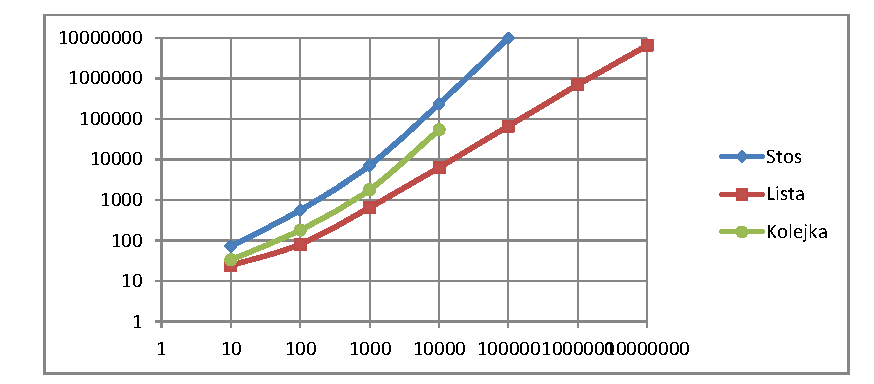
\includegraphics[width=14cm]{Wykres.pdf}
		\caption{Wykres złożoności obliczeniowej.}
	 \end{figure}
	 \section{Komentarz}
	 	Do utworzenia dokumentacji wykorzystano system Doxygen.
	 	Funkcja pomiaru czasu dla systemu Windows pobrana ze strony dr. J. Mierzwy. Program skompilowano w środowisku Code::Blocks. Do stworzonia wykresu posłużono się pakietem MS Excel, sprawozdanie napisano uzywając systemu \LaTeX.
\end{document}